\documentclass[10pt,twocolumn]{article}

\usepackage[a4paper,margin=18mm,columnsep=7mm]{geometry}
\usepackage{fontspec}
\setmainfont{TeX Gyre Termes}
\setsansfont{TeX Gyre Heros}
\usepackage{amsmath}
\usepackage{booktabs}
\usepackage{graphicx}
\usepackage{microtype}
\usepackage{xcolor}
\usepackage{xurl}
\usepackage[hidelinks]{hyperref}
\usepackage[font=small,labelfont=bf]{caption}

\definecolor{ink}{HTML}{333331}
\definecolor{linkblue}{HTML}{2A78D6}
\hypersetup{colorlinks=true,linkcolor=ink,citecolor=linkblue,urlcolor=linkblue}
\setlength{\parindent}{1em}
\setlength{\parskip}{0pt}
\renewcommand{\thefootnote}{\fnsymbol{footnote}}

% Generated from src/pourbase/data/pourbase.sqlite; do not edit by hand.
\newcommand{\DatasetVersion}{1.0.0}
\newcommand{\SpeciesCount}{460}
\newcommand{\SystemCount}{74}
\newcommand{\GibbsCount}{454}
\newcommand{\EntropyCount}{388}
\newcommand{\EnthalpyCount}{293}
\newcommand{\ReportedValueCount}{1412}
\newcommand{\RecommendedValueCount}{1135}
\newcommand{\SourceRecordCount}{400}
\newcommand{\DistinctCitationCount}{72}
\newcommand{\PhaseRecordCount}{126}
\newcommand{\ResolvedPhaseCount}{118}
\newcommand{\MPMatchCount}{105}
\newcommand{\MPEnergyCount}{299}
\newcommand{\FallbackCount}{6}
\newcommand{\WarningCount}{236}
\newcommand{\LigandCount}{5}
\newcommand{\AqueousSpeciesCount}{255}
\newcommand{\SolidSpeciesCount}{194}
\newcommand{\GasSpeciesCount}{9}
\newcommand{\LiquidSpeciesCount}{2}
\newcommand{\GibbsCoveragePercent}{98.7\%}
\newcommand{\EntropyCoveragePercent}{84.3\%}
\newcommand{\EnthalpyCoveragePercent}{63.7\%}
\newcommand{\VerifiedGibbsCount}{328}
\newcommand{\ReferenceGibbsCount}{74}
\newcommand{\EstimatedGibbsCount}{52}
\newcommand{\GibbsGapCount}{6}
\newcommand{\MPDatabaseVersion}{2026.04.13}
\newcommand{\MPEnthalpyRtwoCount}{90}
\newcommand{\MPEnthalpyRtwoMAE}{0.085}
\newcommand{\MPGibbsRtwoCount}{93}
\newcommand{\MPGibbsRtwoMAE}{0.171}


\title{An experimental thermodynamic database and Python toolkit\\for aqueous stability diagrams}
\author{}
\date{}

\begin{document}
\maketitle
\vspace{-2.5em}

\begin{abstract}
We present version \DatasetVersion{} of a source-linked SQLite thermodynamic database and a small
Python package for calculating single-element Pourbaix diagrams. The database contains
\SpeciesCount{} species across \SystemCount{} supported elemental systems at 298.15 K and 1 bar.
Recommended Gibbs energies are available for \GibbsCount{} species, with each value linked to a
scientific source, location, status, and uncertainty when reported. Earlier reported values remain
available alongside the recommended calculation value. The package supports fixed activities,
closed metal mass balance, activity corrections, ligand and gas reservoirs, concentration sweeps,
Boltzmann-like visualization, and direct comparison with the Materials Project. The database,
calculation code, desktop application, figures, and figure data are distributed together
as a reproducible publication bundle.
\end{abstract}

\section{Purpose}

Pourbaix diagrams summarize the thermodynamically preferred aqueous, solid, liquid, or gaseous
form of an element as a function of pH and electrode potential \cite{method-pourbaix}. Their result
depends directly on the thermochemical values and chemical identities supplied to the calculation.
The aim of this work is to make that input inspectable. A user can trace a plotted domain back to
the selected Gibbs energy, the retained alternatives, the physical phase, and the exact source
location.

The release has two connected parts. The SQLite file is the scientific record. The Python package
reads that file without modifying it and turns the selected records into diagrams, tables, balanced
reactions, and machine-readable grids. A desktop application exposes the same backend.

\section{Database}

\subsection{Evidence model}

The \texttt{species} table defines chemical identity, charge, phase, stoichiometry, and the
coefficients needed by the electrochemical calculation. The \texttt{reported\_thermochemistry}
table retains \ReportedValueCount{} sourced observations. The \texttt{thermochemistry} table holds
one documented recommendation for each usable property, giving \RecommendedValueCount{}
calculation-facing values in total. Recommendations are selected only after checking the formula,
phase or polymorph, standard state, temperature, pressure, and source traceability. Alternative
reports remain queryable and are not averaged automatically.

The source layer contains \SourceRecordCount{} value-specific records representing
\DistinctCitationCount{} distinct citation strings. Every source record is used by at least one
thermochemical value, warning, or ligand definition. The complete source bibliography appears at
the end of this paper; exact table, page, or database-row locations remain attached to the SQLite
records.

\begin{table}[t]
\caption{Core contents generated directly from the release database.}
\label{tab:contents}
\centering
\begin{tabular}{lr}
\toprule
Item & Count \\
\midrule
Species & \SpeciesCount \\
Supported elemental systems & \SystemCount \\
Recommended Gibbs energies & \GibbsCount \\
Recommended entropies & \EntropyCount \\
Formation enthalpies & \EnthalpyCount \\
Source records & \SourceRecordCount \\
Phase-identity records & \PhaseRecordCount \\
Materials Project phase matches & \MPMatchCount \\
Materials Project energy rows & \MPEnergyCount \\
\bottomrule
\end{tabular}
\end{table}

\subsection{Coverage and phase identity}

Figure~\ref{fig:overview} summarizes the release. It includes \AqueousSpeciesCount{} aqueous
species, \SolidSpeciesCount{} solids, \GasSpeciesCount{} gases, and \LiquidSpeciesCount{} liquids.
Gibbs energies cover \GibbsCoveragePercent{} of all species, entropy covers
\EntropyCoveragePercent{}, and formation enthalpy covers \EnthalpyCoveragePercent{}. Of the Gibbs
entries, \VerifiedGibbsCount{} are source-verified values, \ReferenceGibbsCount{} are elemental
reference states, and \EstimatedGibbsCount{} are explicitly labelled source-verified estimates.
\GibbsGapCount{} solid records retain an experimental evidence gap. Their optional computational estimates are
stored in a separate fallback table and never replace an experimental recommendation.

Crystalline identity is recorded independently from thermochemistry. The release includes
\PhaseRecordCount{} phase records, of which \ResolvedPhaseCount{} have a resolved identity or a
resolved identity with a thermochemical gap. Accepted links connect \MPMatchCount{} experimental
solid records to Materials Project structures. Formula agreement alone is insufficient for these
links; the recorded evidence includes the phase description, space group when known, match
confidence, and notes on ambiguity.

\begin{figure*}[t]
\centering
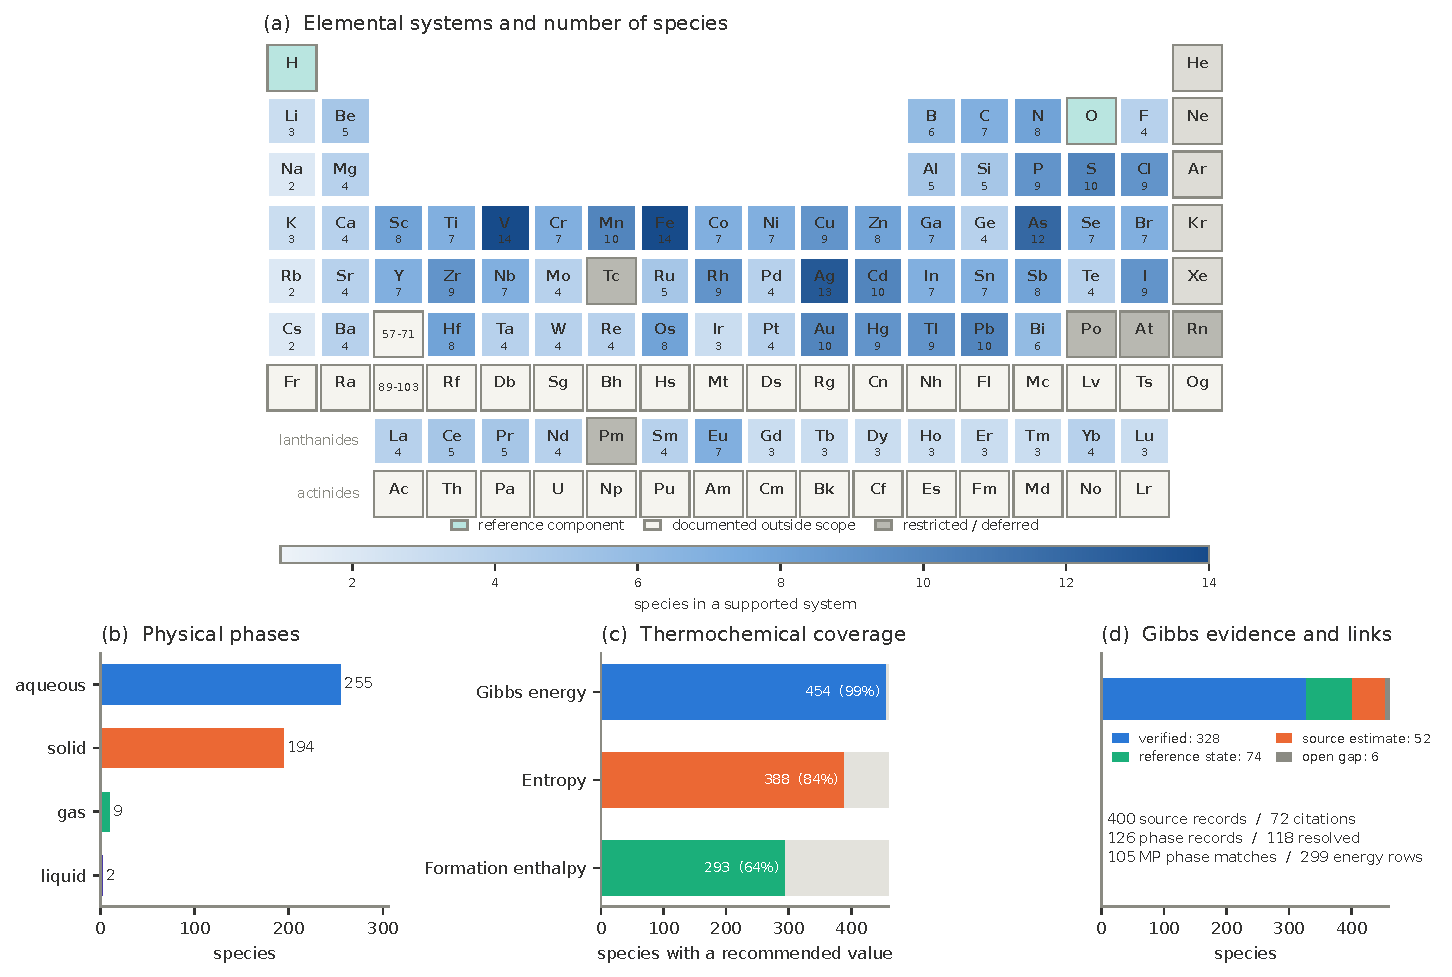
\includegraphics[width=\textwidth]{figures/dataset-overview.pdf}
\caption{Database coverage. (a) Every position in the periodic table has a documented coverage
status; supported systems are colored by their number of species. (b) Species by physical phase.
(c) Availability of the three principal thermochemical properties. Pale bars show the full set of
\SpeciesCount{} species. (d) Evidence status of the recommended Gibbs-energy field and the links
to sources, phases, and Materials Project calculations. All counts are generated from the bundled
SQLite file.}
\label{fig:overview}
\end{figure*}

\section{Calculation model}

The fixed-activity engine compares the transformed Gibbs energy of every included species on a pH
and potential grid. For species $i$, the implemented quantity per mole of the selected element is

\begin{equation}
\begin{aligned}
\widetilde G_i ={}& \frac{\Delta_{\mathrm f}G_i^\circ}{n_{M,i}}
- \frac{n_{O,i}}{n_{M,i}}G_{\mathrm{H_2O}}^\circ \\
&- n_{H,i}RT\ln(10)\,\mathrm{pH}
- n_{e,i}F E + \Delta G_{\mathrm{activity},i},
\end{aligned}
\end{equation}

where the stored stoichiometric coefficients define the proton, electron, water, ligand, and gas
terms. The species with the lowest transformed Gibbs energy defines each domain. Aqueous activities
and gas fugacities are dimensionless relative to 1 mol L$^{-1}$ and 1 bar, respectively. An optional
Davies model supplies aqueous activity coefficients up to 0.1 mol L$^{-1}$ background ionic
strength \cite{method-davies}.

The closed-inventory solver conserves the selected element between dissolved species and a
precipitating solid. It reports the dominant species, dissolved concentration, precipitated
fraction, and full species-fraction grid. The Boltzmann-like view uses

\begin{equation}
w_i = \frac{\exp[-(\widetilde G_i-\widetilde G_{\min})/(sRT)]}
{\sum_j \exp[-(\widetilde G_j-\widetilde G_{\min})/(sRT)]}.
\end{equation}

This soft-minimum view displays energetic competition around sharp domain boundaries. Its weights
are a visualization over the supplied entries. Conserved phase amounts come from the mass-balance
solver.

Figure~\ref{fig:showcase} compares the experimental iron diagram directly with the official
Materials Project workflow under the same grid and aqueous activity. The third panel compares
thermodynamic identities, matching solids by hydrogen and oxygen composition per metal and aqueous
species by their proton and electron coefficients. This recognizes equivalent chemical domains
across different labels while preserving differences such as Fe$_3$O$_4$ versus FeO.

\begin{figure*}[t]
\centering
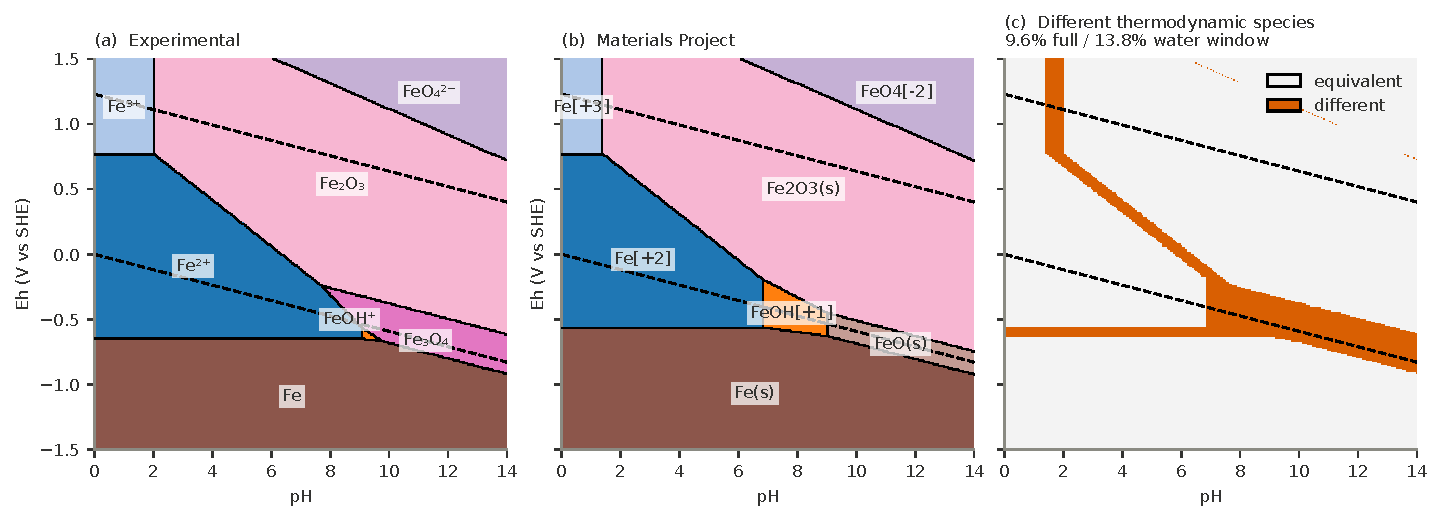
\includegraphics[width=\textwidth]{figures/calculation-showcase.pdf}
\caption{Iron Pourbaix comparison at 298.15 K, 1 bar, and aqueous activity $10^{-6}$. The dashed
lines delimit water stability. (a) Domains calculated from the experimental Gibbs database.
(b) Domains from the official Materials Project workflow, cached with database version
\MPDatabaseVersion{}. (c) Grid cells with different thermodynamic identities. The versioned MP
phase inputs, software versions, comparison mask summary, and changed phase pairs are included with
the paper assets.}
\label{fig:showcase}
\end{figure*}

\section{Comparison with calculated materials data}

The release stores \MPEnergyCount{} method-specific Materials Project energy rows for
\MPMatchCount{} phase-matched experimental records. The stored database version is
\MPDatabaseVersion{}.
Materials Project provides the calculated solid entries and formalism for first-principles aqueous
stability calculations \cite{method-persson,method-jain,method-horton,method-singh}. The package can
also request a current official Materials Project Pourbaix diagram through the user's own API key.

Figure~\ref{fig:mp} compares each calculated formation energy with the phase-matched experimental
formation enthalpy and Gibbs energy. Formation enthalpy is the closer comparison to the nominally
0 K DFT formation energy. For r2SCAN, the mean absolute enthalpy residual is
\MPEnthalpyRtwoMAE{} eV atom$^{-1}$ across \MPEnthalpyRtwoCount{} plotted calculations. The
corresponding Gibbs residual is \MPGibbsRtwoMAE{} eV atom$^{-1}$ across \MPGibbsRtwoCount{}
calculations. The latter also contains finite-temperature entropy contributions. These plots
therefore measure agreement between documented phases under stated normalizations; they do not
serve as interchangeable definitions of the same thermodynamic quantity. The optional 300 K
fallbacks use the published SISSO Gibbs descriptor \cite{method-bartel} and remain clearly marked
as computational.

\begin{figure*}[t]
\centering
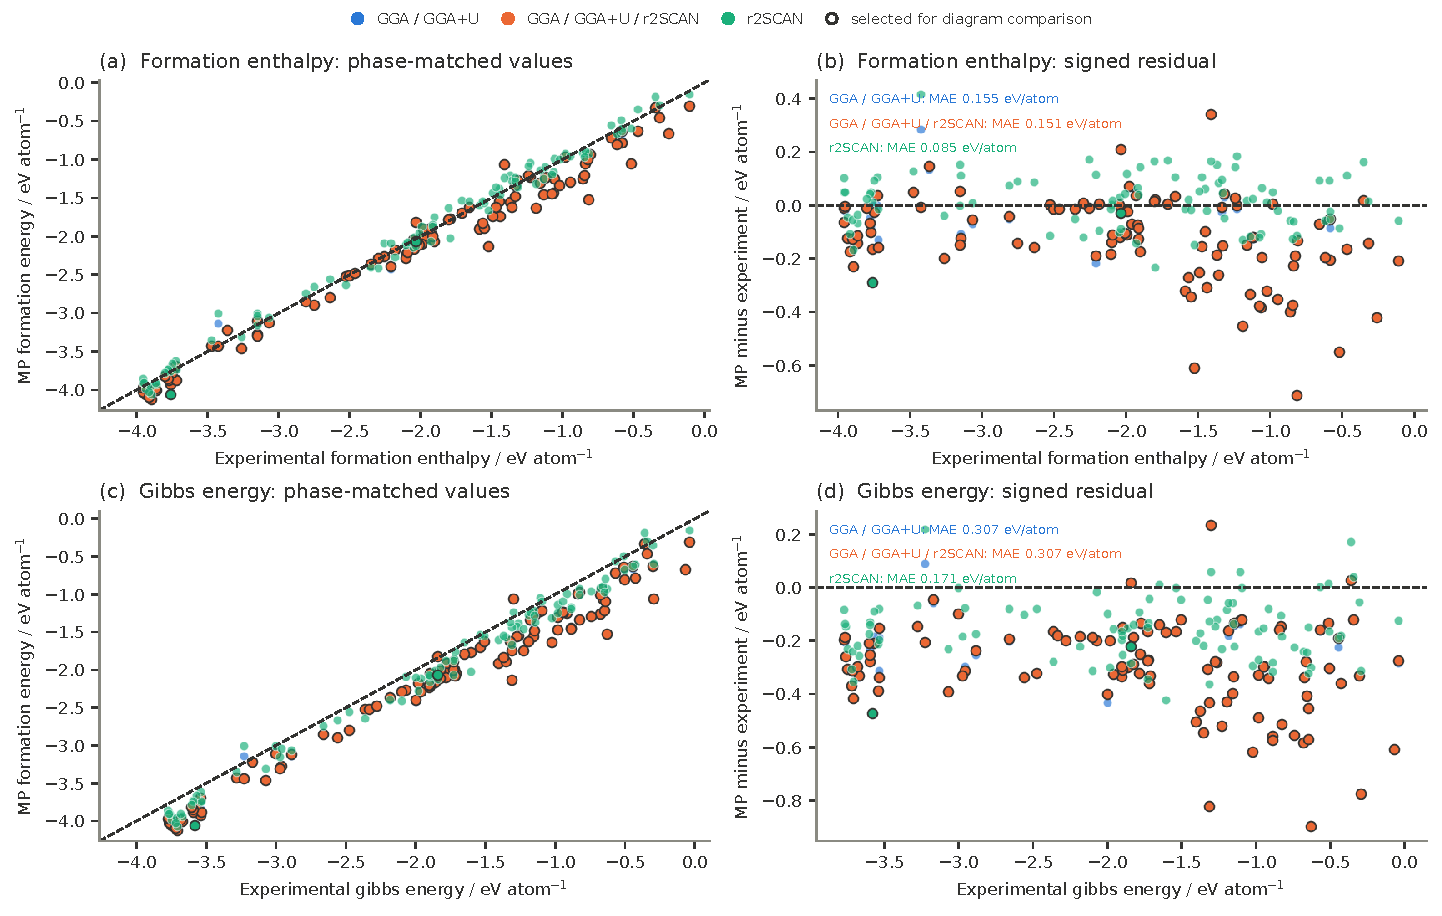
\includegraphics[width=\textwidth]{figures/mp-thermochemistry.pdf}
\caption{Direct comparison between experimental values and phase-matched Materials Project
formation energies, normalized to eV per atom. Left panels show equality plots; right panels show
the signed residual, defined as Materials Project minus experiment. A dark marker edge identifies
the calculation selected for diagram comparison. The plotted rows, MP identifiers, methods,
database version, retrieval dates, and numerical metrics ship with the package.}
\label{fig:mp}
\end{figure*}

\section{Software and reproducibility}

The Python package uses NumPy and Matplotlib \cite{software-numpy,software-matplotlib}. Its public
objects cover database access, conditions, fixed-activity and mass-balanced engines, speciation,
concentration conversion, sweeps, plotting, and official Materials Project comparison. Both the
command-line interface and desktop application call those objects. Each generated result contains
the calculation settings, included and excluded species, warnings, sources, and grid data.

The manuscript assets are regenerated with one command:

\begin{verbatim}
make -C paper
\end{verbatim}

The script reads only \texttt{src/pourbase/data/pourbase.sqlite} and the versioned Materials Project comparison
CSV and JSON files. It writes the statistics JSON, per-system CSV, LaTeX count macros, complete
source bibliography, and all three figures before compiling this manuscript.

\section{Scope}

Version \DatasetVersion{} evaluates single-element systems at 298.15 K and 1 bar. It does not
extrapolate thermochemistry with temperature because consistent heat-capacity information is not
yet available across competing species. Multi-element phase competition, kinetic persistence,
surface energy, particle size, explicit solvent structure, and electrochemical overpotential lie
outside the present equilibrium model. Gas-containing systems use fixed fugacity; the closed mass
balance currently covers systems without a gas phase.

The database exposes these limits through statuses and warnings. Calculations require complete
recommended Gibbs data by default. A user can deliberately allow a documented gap or select the
separate experimental-then-Materials-Project fallback policy. This keeps exploratory calculations
visible and reproducible.

\section{Data availability}

The release bundle contains the SQLite database, Python source, tests, desktop application, manuscript source, generated statistics, figure data, and vector figures. Data
records retain their original citations and source locations. Materials Project extracts and
derived comparisons retain MP identifiers, versions, and attribution. The accompanying
\texttt{THIRD\_PARTY\_NOTICES.md} describes source-specific attribution, while
\texttt{DATA\_DICTIONARY.md} defines every table and unit.

% Generated from the sources table; do not edit by hand.
\begin{thebibliography}{99}
\bibitem{method-pourbaix} Pourbaix, M. Atlas of Electrochemical Equilibria in Aqueous Solutions, 2nd English ed., National Association of Corrosion Engineers (1974).
\bibitem{method-davies} Davies, C. W. The extent of dissociation of salts in water. Part VIII. An equation for the mean ionic activity coefficient of an electrolyte. Journal of the Chemical Society, 2093-2098 (1938).
\url{https://doi.org/10.1039/JR9380002093}
\bibitem{method-persson} Persson, K. A. et al. Prediction of solid-aqueous equilibria: Scheme to combine first-principles calculations of solids with experimental aqueous states. Physical Review B 85, 235438 (2012).
\url{https://doi.org/10.1103/PhysRevB.85.235438}
\bibitem{method-jain} Jain, A. et al. Commentary: The Materials Project: A materials genome approach to accelerating materials innovation. APL Materials 1, 011002 (2013).
\url{https://doi.org/10.1063/1.4812323}
\bibitem{method-horton} Horton, M. K. et al. Accelerated data-driven materials science with the Materials Project. Nature Materials 24, 1522-1532 (2025).
\url{https://doi.org/10.1038/s41563-025-02272-0}
\bibitem{method-singh} Singh, A. K. et al. Electrochemical stability of metastable materials. Chemistry of Materials 29, 10159-10167 (2017).
\url{https://doi.org/10.1021/acs.chemmater.7b03980}
\bibitem{method-bartel} Bartel, C. J. et al. Physical descriptor for the Gibbs energy of inorganic crystalline solids and temperature-dependent materials chemistry. Nature Communications 9, 4168 (2018).
\url{https://doi.org/10.1038/s41467-018-06682-4}
\bibitem{software-numpy} Harris, C. R. et al. Array programming with NumPy. Nature 585, 357-362 (2020).
\url{https://doi.org/10.1038/s41586-020-2649-2}
\bibitem{software-matplotlib} Hunter, J. D. Matplotlib: A 2D graphics environment. Computing in Science and Engineering 9, 90-95 (2007).
\url{https://doi.org/10.1109/MCSE.2007.55}
\bibitem{data-source-001} Ashcroft, S. J. and Schwarzmann, E. Standard enthalpy of formation of crystalline gold(III) oxide. Journal of the Chemical Society, Faraday Transactions 1 68, 1360-1361 (1972). DOI: 10.1039/F19726801360.
Database link: \url{https://doi.org/10.1039/F19726801360}
\textit{Used by 1 source record in version \DatasetVersion.}
\bibitem{data-source-002} Bard, A. J., Parsons, R. \& Jordan, J. (eds.). Standard Potentials in Aqueous Solution. IUPAC/Marcel Dekker (1985), chapter 16, pp. 457-459.
Database link: \url{https://www.routledge.com/Standard-Potentials-in-Aqueous-Solution/Bard-Parsons-Jordan/p/book/9780824772918}
\textit{Used by 1 source record in version \DatasetVersion.}
\bibitem{data-source-003} Bard, A. J., Parsons, R. and Jordan, J. (eds.). Standard Potentials in Aqueous Solution. IUPAC/Marcel Dekker (1985).
Database link: \url{https://www.routledge.com/Standard-Potentials-in-Aqueous-Solution/Bard-Parsons-Jordan/p/book/9780824772918}
\textit{Used by 4 source records in version \DatasetVersion.}
\bibitem{data-source-004} Barner, H. E. and Scheuerman, R. V. Handbook of Thermochemical Data for Compounds and Aqueous Species. Wiley, New York (1978). Value transcribed through the Materials Project ion-reference dataset.
Database link: \url{https://docs.materialsproject.org/methodology/materials-methodology/aqueous-stability-pourbaix}
\textit{Used by 1 source record in version \DatasetVersion.}
\bibitem{data-source-005} Benezeth, P. et al. Gallium speciation in aqueous solution: Experimental study and modelling: Part 2. Geochimica et Cosmochimica Acta 61, 1345-1357 (1997). DOI: 10.1016/S0016-7037(97)00012-4.
Database link: \url{https://doi.org/10.1016/S0016-7037(97)00012-4}
\textit{Used by 1 source record in version \DatasetVersion.}
\bibitem{data-source-006} Beverskog, B. and Puigdomenech, I. Revised Pourbaix diagrams for zinc at 25-300 degrees C. Corrosion Science 39, 107-114 (1997).
Database link: \url{https://doi.org/10.1016/S0010-938X(97)89246-3}
\textit{Used by 1 source record in version \DatasetVersion.}
\bibitem{data-source-007} Bratsch, S. G. Standard Electrode Potentials and Temperature Coefficients in Water at 298.15 K. Journal of Physical and Chemical Reference Data 18, 1-21 (1989).
Database link: \url{https://doi.org/10.1063/1.555839}
\textit{Used by 2 source records in version \DatasetVersion.}
\bibitem{data-source-008} Bricker, O. P. Some stability relations in the system Mn-O2-H2O at 25 C and one atmosphere total pressure. American Mineralogist 50, 1296-1354 (1965).
Database link: \url{https://msaweb.org/AmMin/AM50/AM50_1296.pdf}
\textit{Used by 2 source records in version \DatasetVersion.}
\bibitem{data-source-009} Chase, M. W., Jr. NIST-JANAF Thermochemical Tables, Fourth Edition, Journal of Physical and Chemical Reference Data, Monograph 9 (1998), table Ca-020.
Database link: \url{https://janaf.nist.gov/tables/Ca-020.html}
\textit{Used by 1 source record in version \DatasetVersion.}
\bibitem{data-source-010} Chase, M. W., Jr. NIST-JANAF Thermochemical Tables, Fourth Edition, Journal of Physical and Chemical Reference Data, Monograph 9 (1998), table Cr-016. DOI: 10.18434/T42S31.
Database link: \url{https://janaf.nist.gov/tables/Cr-016.html}
\textit{Used by 1 source record in version \DatasetVersion.}
\bibitem{data-source-011} Chase, M. W., Jr. NIST-JANAF Thermochemical Tables, Fourth Edition, Journal of Physical and Chemical Reference Data, Monograph 9 (1998), table Cu-015.
Database link: \url{https://janaf.nist.gov/tables/Cu-015.html}
\textit{Used by 1 source record in version \DatasetVersion.}
\bibitem{data-source-012} Chase, M. W., Jr. NIST-JANAF Thermochemical Tables, Fourth Edition, Journal of Physical and Chemical Reference Data, Monograph 9 (1998), table Cu-019.
Database link: \url{https://janaf.nist.gov/tables/Cu-019.html}
\textit{Used by 1 source record in version \DatasetVersion.}
\bibitem{data-source-013} Chase, M. W., Jr. NIST-JANAF Thermochemical Tables, Fourth Edition, Journal of Physical and Chemical Reference Data, Monograph 9 (1998), table Fe-030.
Database link: \url{https://janaf.nist.gov/tables/Fe-030.html}
\textit{Used by 1 source record in version \DatasetVersion.}
\bibitem{data-source-014} Chase, M. W., Jr. NIST-JANAF Thermochemical Tables, Fourth Edition, Journal of Physical and Chemical Reference Data, Monograph 9 (1998), table Fe-032.
Database link: \url{https://janaf.nist.gov/tables/Fe-032.html}
\textit{Used by 1 source record in version \DatasetVersion.}
\bibitem{data-source-015} Chase, M. W., Jr. NIST-JANAF Thermochemical Tables, Fourth Edition, Journal of Physical and Chemical Reference Data, Monograph 9 (1998), table H-057.
Database link: \url{https://janaf.nist.gov/tables/H-057.html}
\textit{Used by 1 source record in version \DatasetVersion.}
\bibitem{data-source-016} Chase, M. W., Jr. NIST-JANAF Thermochemical Tables, Fourth Edition, Journal of Physical and Chemical Reference Data, Monograph 9 (1998), table O-005.
Database link: \url{https://janaf.nist.gov/tables/O-005.html}
\textit{Used by 1 source record in version \DatasetVersion.}
\bibitem{data-source-017} Chase, M. W., Jr. NIST-JANAF Thermochemical Tables, Fourth Edition, Journal of Physical and Chemical Reference Data, Monograph 9 (1998), table O-033.
Database link: \url{https://janaf.nist.gov/tables/O-033.html}
\textit{Used by 1 source record in version \DatasetVersion.}
\bibitem{data-source-018} Chase, M. W., Jr. NIST-JANAF Thermochemical Tables, Fourth Edition, Journal of Physical and Chemical Reference Data, Monograph 9 (1998), table O-043.
Database link: \url{https://janaf.nist.gov/tables/O-043.html}
\textit{Used by 1 source record in version \DatasetVersion.}
\bibitem{data-source-019} Chase, M. W., Jr. NIST-JANAF Thermochemical Tables, Fourth Edition, Journal of Physical and Chemical Reference Data, Monograph 9 (1998), table O-070.
Database link: \url{https://janaf.nist.gov/tables/O-070.html}
\textit{Used by 1 source record in version \DatasetVersion.}
\bibitem{data-source-020} Chase, M. W., Jr. NIST-JANAF Thermochemical Tables, Fourth Edition. Journal of Physical and Chemical Reference Data, Monograph 9 (1998).
Database link: \url{https://janaf.nist.gov/tables/Ba-025.html}
\textit{Used by 5 source records in version \DatasetVersion.}
\bibitem{data-source-021} Chase, M. W., Jr. NIST-JANAF Thermochemical Tables, Fourth Edition. Journal of Physical and Chemical Reference Data, Monograph 9 (1998). DOI: 10.18434/T42S31.
Database link: \url{https://janaf.nist.gov/tables/Al-001.html}
\textit{Used by 28 source records in version \DatasetVersion.}
\bibitem{data-source-022} Chase, M. W., Jr. NIST-JANAF Thermochemical Tables, Fourth Edition. Journal of Physical and Chemical Reference Data, Monograph 9 (1998). NIST Standard Reference Database 13. DOI: 10.18434/T42S31.
Database link: \url{https://janaf.nist.gov/tables/Al-096.html}
\textit{Used by 7 source records in version \DatasetVersion.}
\bibitem{data-source-023} Chatillon, C., Nuta, I., Roki, F.-Z. and Fischer, E. Chemical thermodynamics of RuO2(s). Journal of Nuclear Materials 509 (2018) 742-751.
Database link: \url{https://doi.org/10.1016/j.jnucmat.2018.05.060}
\textit{Used by 1 source record in version \DatasetVersion.}
\bibitem{data-source-024} Cox, J. D., Wagman, D. D. and Medvedev, V. A. CODATA Key Values for Thermodynamics. Hemisphere Publishing Corporation (1984), as served by NIST SRD 69.
Database link: \url{https://webbook.nist.gov/cgi/cbook.cgi?ID=C7440224&Mask=2&Units=SI}
\textit{Used by 2 source records in version \DatasetVersion.}
\bibitem{data-source-025} Filella, M. and May, P. M. The aqueous solution thermodynamics of tantalum under conditions of environmental and biological interest. Applied Geochemistry 109, 104402 (2019).
Database link: \url{https://doi.org/10.1016/j.apgeochem.2019.104402}
\textit{Used by 1 source record in version \DatasetVersion.}
\bibitem{data-source-026} Gamsjager, H. et al. Chemical Thermodynamics of Nickel. OECD Nuclear Energy Agency, Chemical Thermodynamics Series Volume 6 (2005).
Database link: \url{https://tdb.oecd-nea.org/dbtdb/pubs/vol6-nickel.pdf}
\textit{Used by 2 source records in version \DatasetVersion.}
\bibitem{data-source-027} Gamsjager, H., Gajda, T., Sangster, J., Saxena, S. K. and Voigt, W. Chemical Thermodynamics of Tin. OECD Nuclear Energy Agency, Chemical Thermodynamics Series Volume 12 (2012).
Database link: \url{https://www.oecd.org/content/dam/oecd/en/publications/reports/2012/12/chemical-thermodynamics-of-tin-volume-12_g1g39522/9789264992061-en.pdf}
\textit{Used by 1 source record in version \DatasetVersion.}
\bibitem{data-source-028} Gamsjäger, H. et al. Chemical Thermodynamics of Nickel. OECD Nuclear Energy Agency, Chemical Thermodynamics Series Volume 6 (2005).
Database link: \url{https://www.oecd-nea.org/upload/docs/application/pdf/2020-09/chemical_thermodynamics_of_nickel_volume_6.pdf}
\textit{Used by 1 source record in version \DatasetVersion.}
\bibitem{data-source-029} Hem, J. D., Roberson, C. E. and Lind, C. J. Thermodynamic stability of CoOOH and its coprecipitation with manganese. Geochimica et Cosmochimica Acta 49, 801-810 (1985). DOI: 10.1016/0016-7037(85)90173-5.
Database link: \url{https://www.usgs.gov/publications/thermodynamic-stability-coooh-and-its-coprecipitation-manganese}
\textit{Used by 1 source record in version \DatasetVersion.}
\bibitem{data-source-030} Hummel, W. and Thoenen, T. The PSI Chemical Thermodynamic Database 2020. Nagra Technical Report NTB 21-03 (2023).
Database link: \url{https://nagra.ch/wp-content/uploads/2023/05/NTB-21-03.pdf}
\textit{Used by 1 source record in version \DatasetVersion.}
\bibitem{data-source-031} IUPAC. "reference state" in Compendium of Chemical Terminology, 5th ed. (2025). DOI: 10.1351/goldbook.R05233.
Database link: \url{https://goldbook.iupac.org/terms/view/R05233}
\textit{Used by 1 source record in version \DatasetVersion.}
\bibitem{data-source-032} Jacob, K. T. and Prusty, D. Thermodynamic Properties of RhO2. Journal of Alloys and Compounds 507, L17-L20 (2010).
Database link: \url{https://doi.org/10.1016/j.jallcom.2010.07.179}
\textit{Used by 1 source record in version \DatasetVersion.}
\bibitem{data-source-033} Jacob, K. T., Mishra, S. and Waseda, Y. Refinement of the Thermodynamic Properties of Ruthenium Dioxide and Osmium Dioxide. Journal of the American Ceramic Society 83, 1745-1752 (2000).
Database link: \url{https://doi.org/10.1111/j.1151-2916.2000.tb01459.x}
\textit{Used by 1 source record in version \DatasetVersion.}
\bibitem{data-source-034} Jacob, K. T., Uda, T., Okabe, T. H. and Waseda, Y. The Standard Enthalpy and Entropy of Formation of Rh2O3: A Third-Law Optimization. High Temperature Materials and Processes 19, 11-16 (2000).
Database link: \url{https://doi.org/10.1515/HTMP.2000.19.1.11}
\textit{Used by 1 source record in version \DatasetVersion.}
\bibitem{data-source-035} Johnson, D. A. and Nelson, P. G. Improvements in Estimated Entropies and Related Thermodynamic Data for Aqueous Metal Ions. Inorganic Chemistry 51, 6116-6128 (2012).
Database link: \url{https://doi.org/10.1021/ic3000334}
\textit{Used by 1 source record in version \DatasetVersion.}
\bibitem{data-source-036} Jordan, N. et al. A critical review of the solution chemistry, solubility, and thermodynamics of europium: Recent advances on the Eu(III) hydrolysis. Coordination Chemistry Reviews 510, 215702 (2024).
Database link: \url{https://doi.org/10.1016/j.ccr.2024.215702}
\textit{Used by 1 source record in version \DatasetVersion.}
\bibitem{data-source-037} Kim, K. J. et al. Real-Time Monitoring of the Thermal Effect for the Redox Flow Battery by an Infrared Thermal Imaging Technology. Energies 13, 6717 (2020).
Database link: \url{https://doi.org/10.3390/en13246717}
\textit{Used by 1 source record in version \DatasetVersion.}
\bibitem{data-source-038} Kirklin, D. R. Properties of Materials and Systems of Importance to Environmental Fates and Remediation. III. Review of Previous Thermodynamic Property Values for Chromium and Some of its Compounds. Journal of Physical and Chemical Reference Data 28, 1675-1705 (1999).
Database link: \url{https://doi.org/10.1063/1.556053}
\textit{Used by 1 source record in version \DatasetVersion.}
\bibitem{data-source-039} Kleykamp, H. and Paneth, E. Gibbs energy of formation of iridium dioxide. Journal of Inorganic and Nuclear Chemistry 35 (1973).
Database link: \url{https://doi.org/10.1016/0022-1902(73)80559-7}
\textit{Used by 1 source record in version \DatasetVersion.}
\bibitem{data-source-040} Lemire, R. J. et al. Chemical Thermodynamics of Iron, Part 1. OECD Nuclear Energy Agency, NEA No. 6355 (2013).
Database link: \url{https://www.oecd-nea.org/upload/docs/application/pdf/2019-12/6355-vol13a-iron.pdf}
\textit{Used by 2 source records in version \DatasetVersion.}
\bibitem{data-source-041} Linstrom, P.J. and Mallard, W.G. (Eds.), NIST Chemistry WebBook, NIST Standard Reference Database Number 69. National Institute of Standards and Technology, Gaithersburg MD. Retrieved 2025.
Database link: \url{https://webbook.nist.gov/chemistry/}
\textit{Used by 1 source record in version \DatasetVersion.}
\bibitem{data-source-042} Merli, L., Lambert, B. and Fuger, J. Thermochemistry of lanthanum, neodymium, samarium and americium trihydroxides and their relation to the corresponding hydroxycarbonates. Journal of Nuclear Materials 247, 172-176 (1997).
Database link: \url{https://doi.org/10.1016/S0022-3115(97)00044-5}
\textit{Used by 1 source record in version \DatasetVersion.}
\bibitem{data-source-043} Migdisov, A., Williams-Jones, A. E., Brugger, J. and Caporuscio, F. A. Hydrothermal transport, deposition, and fractionation of the REE: Experimental data and thermodynamic calculations. Chemical Geology 439, 13-42 (2016). DOI 10.1016/j.chemgeo.2016.06.005. Diakonov, I. I., Tagirov, B. R. and Ragnarsdottir, K. V. Standard thermodynamic properties and heat capacity equations for rare earth element hydroxides: I. La(OH)3(s) and Nd(OH)3(s). Radiochimica Acta 81, 107-116 (1998).
Database link: \url{https://www.osti.gov/servlets/purl/1351190}
\textit{Used by 2 source records in version \DatasetVersion.}
\bibitem{data-source-044} Misawa, T. The thermodynamic consideration for Fe-H2O system at 25 degrees C. Corrosion Science 13, 659-676 (1973).
Database link: \url{https://doi.org/10.1016/S0010-938X(73)80037-X}
\textit{Used by 1 source record in version \DatasetVersion.}
\bibitem{data-source-045} NIST Chemistry WebBook, SRD 69. Nitrogen Henry's-law data at 298.15 K, compiled by Rolf Sander.
Database link: \url{https://webbook.nist.gov/cgi/cbook.cgi?ID=C7727379&Mask=10}
\textit{Used by 1 source record in version \DatasetVersion.}
\bibitem{data-source-046} Navrotsky, A. et al. Thermodynamics of solid phases containing rare earth oxides. Journal of Chemical Thermodynamics 88, 126-141 (2015).
Database link: \url{https://doi.org/10.1016/j.jct.2015.04.008}
\textit{Used by 2 source records in version \DatasetVersion.}
\bibitem{data-source-047} Parker, V. B. and Khodakovskii, I. L. Thermodynamic Properties of the Aqueous Ions (2+ and 3+) of Iron and the Key Compounds of Iron. Journal of Physical and Chemical Reference Data 24, 1699-1745 (1995).
Database link: \url{https://doi.org/10.1063/1.555964}
\textit{Used by 1 source record in version \DatasetVersion.}
\bibitem{data-source-048} Puigdomenech, I. and Taxen, C. Thermodynamic data for copper: Implications for the corrosion of copper under repository conditions. SKB TR-00-13 (2000).
Database link: \url{https://skb.se/upload/publications/pdf/TR-00-13.pdf}
\textit{Used by 2 source records in version \DatasetVersion.}
\bibitem{data-source-049} Robie, R. A. and Hemingway, B. S. Thermodynamic properties of minerals and related substances at 298.15 K and 1 bar pressure and at higher temperatures. U.S. Geological Survey Bulletin 2131 (1995).
Database link: \url{https://doi.org/10.3133/b2131}
\textit{Used by 1 source record in version \DatasetVersion.}
\bibitem{data-source-050} Sassani, D. C. and Shock, E. L. Solubility and transport of platinum-group elements in supercritical fluids: summary and estimates of thermodynamic properties for ruthenium, rhodium, palladium, and platinum solids, aqueous ions, and complexes to 1000 C and 5 kbar. Geochimica et Cosmochimica Acta 62, 2643-2671 (1998). DOI: 10.1016/S0016-7037(98)00049-0. Values transcribed through WORM Database commit a0416d17d60faa03de3c371b9f2726f77a750c34.
Database link: \url{https://raw.githubusercontent.com/worm-portal/WORM-db/a0416d17d60faa03de3c371b9f2726f77a750c34/wrm_data_latest.csv}
\textit{Used by 5 source records in version \DatasetVersion.}
\bibitem{data-source-051} Sassani, D. C. and Shock, E. L. Solubility and transport of platinum-group elements in supercritical fluids: summary and estimates of thermodynamic properties for ruthenium, rhodium, palladium, and platinum solids, aqueous ions, and complexes to 1000 C and 5 kbar. Geochimica et Cosmochimica Acta 62, 2643-2671 (1998). WORM Database snapshot commit a0416d17d60faa03de3c371b9f2726f77a750c34.
Database link: \url{https://doi.org/10.1016/S0016-7037(98)00049-0}
\textit{Used by 3 source records in version \DatasetVersion.}
\bibitem{data-source-052} Schumm, R. H. et al. Selected Values of Chemical Thermodynamic Properties, Tables for the Lanthanide (Rare Earth) Elements. NBS Technical Note 270-7 (1973).
Database link: \url{https://nvlpubs.nist.gov/nistpubs/Legacy/TN/nbstechnicalnote270-7.pdf}
\textit{Used by 1 source record in version \DatasetVersion.}
\bibitem{data-source-053} Schumm, R. H. et al. Selected Values of Chemical Thermodynamic Properties, Tables for the Lanthanide (Rare Earth) Elements. NBS Technical Note 270-7 (1973). Konings, R. J. M., van Miltenburg, J. C. and Van Genderen, A. C. G. Heat capacity and entropy of monoclinic Gd2O3. Journal of Chemical Thermodynamics 37, 1219-1225 (2005).
Database link: \url{https://doi.org/10.1016/j.jct.2005.02.014}
\textit{Used by 1 source record in version \DatasetVersion.}
\bibitem{data-source-054} Shock, E. L., Sassani, D. C., Willis, M. and Sverjensky, D. A. Inorganic species in geologic fluids: Correlations among standard molal thermodynamic properties of aqueous ions and hydroxide complexes. Geochimica et Cosmochimica Acta 61, 907-950 (1997). DOI: 10.1016/S0016-7037(96)00339-0. Values transcribed through WORM Database commit a0416d17d60faa03de3c371b9f2726f77a750c34.
Database link: \url{https://raw.githubusercontent.com/worm-portal/WORM-db/a0416d17d60faa03de3c371b9f2726f77a750c34/wrm_data_latest.csv}
\textit{Used by 23 source records in version \DatasetVersion.}
\bibitem{data-source-055} Shock, E. L., Sassani, D. C., Willis, M. and Sverjensky, D. A. Inorganic species in geologic fluids: Correlations among standard molal thermodynamic properties of aqueous ions and hydroxide complexes. Geochimica et Cosmochimica Acta 61, 907-950 (1997). WORM Database snapshot commit a0416d17d60faa03de3c371b9f2726f77a750c34.
Database link: \url{https://raw.githubusercontent.com/worm-portal/WORM-db/a0416d17d60faa03de3c371b9f2726f77a750c34/wrm_data_latest.csv}
\textit{Used by 12 source records in version \DatasetVersion.}
\bibitem{data-source-056} Shock, E. L., Sassani, D. C., Willis, M. and Sverjensky, D. A. Inorganic species in geologic fluids: correlations among standard molal thermodynamic properties of aqueous ions and hydroxide complexes. Geochimica et Cosmochimica Acta 61, 907-950 (1997). DOI: 10.1016/S0016-7037(96)00339-0. Value transcribed through the saved Materials Project ion-reference dataset.
Database link: \url{https://docs.materialsproject.org/methodology/materials-methodology/aqueous-stability-pourbaix}
\textit{Used by 1 source record in version \DatasetVersion.}
\bibitem{data-source-057} Shock, E. L., Sassani, D. C., Willis, M. and Sverjensky, D. A. Inorganic species in geologic fluids: correlations among standard molal thermodynamic properties of aqueous ions and hydroxide complexes. Geochimica et Cosmochimica Acta 61, 907-950 (1997). WORM Database snapshot commit a0416d17d60faa03de3c371b9f2726f77a750c34.
Database link: \url{https://doi.org/10.1016/S0016-7037(96)00339-0}
\textit{Used by 1 source record in version \DatasetVersion.}
\bibitem{data-source-058} Smirnova, N. N. et al. Low-Temperature Heat Capacity and Standard Entropy of PdO(cr.). Russian Journal of Physical Chemistry A 84, 1851-1855 (2010). DOI: 10.1134/S0036024410110051.
Database link: \url{https://doi.org/10.1134/S0036024410110051}
\textit{Used by 1 source record in version \DatasetVersion.}
\bibitem{data-source-059} Stern, K. H. High Temperature Properties and Decomposition of Inorganic Salts Part 3, Nitrates and Nitrites. Journal of Physical and Chemical Reference Data 1, 747-772 (1972). DOI: 10.1063/1.3253104.
Database link: \url{https://doi.org/10.1063/1.3253104}
\textit{Used by 1 source record in version \DatasetVersion.}
\bibitem{data-source-060} Stuve, J. M. and Ferrante, M. J. Thermodynamic Properties of Rhenium Oxides, 8 to 1,400 K. U.S. Bureau of Mines Report of Investigations 8199 (1976).
Database link: \url{https://stacks.cdc.gov/view/cdc/237634/cdc_237634_DS1.pdf}
\textit{Used by 1 source record in version \DatasetVersion.}
\bibitem{data-source-061} Tagirov, B. R., Baranova, N. N. and Bychkova, Y. V. Thermodynamic properties of platinum chloride complexes in aqueous solutions: derivation of consistent parameters from literature data and experiments on Pt(cr) solubility at 400-475 C and 1 kbar. Geochemistry International 53, 327-340 (2015). CHNOSZ 2.2.0 database extraction.
Database link: \url{https://doi.org/10.1134/S0016702915040084}
\textit{Used by 1 source record in version \DatasetVersion.}
\bibitem{data-source-062} Wagman, D. D. et al. NBS Tables of Chemical Thermodynamic Properties, machine-readable library with erratum values. NIST SRD 13. https://doi.org/10.18434/M32124.
Database link: \url{https://doi.org/10.18434/M32124}
\textit{Used by 1 source record in version \DatasetVersion.}
\bibitem{data-source-063} Wagman, D. D. et al. Selected Values of Chemical Thermodynamic Properties. NBS Technical Note 270 (1968-1971). Value transcribed through the saved Materials Project ion-reference dataset.
Database link: \url{https://docs.materialsproject.org/methodology/materials-methodology/aqueous-stability-pourbaix}
\textit{Used by 2 source records in version \DatasetVersion.}
\bibitem{data-source-064} Wagman, D. D. et al. The NBS Tables of Chemical Thermodynamic Properties. Journal of Physical and Chemical Reference Data 11, Supplement 2 (1982), table 29:Al.
Database link: \url{https://srd.nist.gov/JPCRD/jpcrdS2Vol11.pdf}
\textit{Used by 1 source record in version \DatasetVersion.}
\bibitem{data-source-065} Wagman, D. D. et al. The NBS Tables of Chemical Thermodynamic Properties. Journal of Physical and Chemical Reference Data 11, Supplement 2 (1982), table 33:Zn.
Database link: \url{https://data.nist.gov/od/ds/mds2-2124/NBS_Tables_with_ErratumValues.csv}
\textit{Used by 1 source record in version \DatasetVersion.}
\bibitem{data-source-066} Wagman, D. D. et al. The NBS Tables of Chemical Thermodynamic Properties. Journal of Physical and Chemical Reference Data 11, Supplement 2 (1982), table 39:Ni.
Database link: \url{https://data.nist.gov/od/ds/mds2-2124/NBS_Tables_with_ErratumValues.csv}
\textit{Used by 1 source record in version \DatasetVersion.}
\bibitem{data-source-067} Wagman, D. D. et al. The NBS Tables of Chemical Thermodynamic Properties. Journal of Physical and Chemical Reference Data 11, Supplement 2 (1982), table 44:Ru.
Database link: \url{https://srd.nist.gov/JPCRD/jpcrdS2Vol11.pdf}
\textit{Used by 1 source record in version \DatasetVersion.}
\bibitem{data-source-068} Wagman, D. D. et al. The NBS Tables of Chemical Thermodynamic Properties. Journal of Physical and Chemical Reference Data 11, Supplement 2 (1982).
Database link: \url{https://data.nist.gov/od/ds/mds2-2124/NBS_Tables_with_ErratumValues.csv}
\textit{Used by 36 source records in version \DatasetVersion.}
\bibitem{data-source-069} Wagman, D. D. et al. The NBS Tables of Chemical Thermodynamic Properties. Journal of Physical and Chemical Reference Data 11, Supplement 2 (1982). Digitized dataset with errata, NIST DOI 10.18434/M32124.
Database link: \url{https://doi.org/10.18434/M32124}
\textit{Used by 105 source records in version \DatasetVersion.}
\bibitem{data-source-070} Wagman, D. D. et al. The NBS Tables of Chemical Thermodynamic Properties. Journal of Physical and Chemical Reference Data 11, Supplement 2 (1982). Digitized with errata by Reed, J. J. (2020), NIST DOI 10.18434/M32124.
Database link: \url{https://data.nist.gov/od/ds/mds2-2124/NBS_Tables_with_ErratumValues.csv}
\textit{Used by 44 source records in version \DatasetVersion.}
\bibitem{data-source-071} Wagman, D. D. et al. The NBS Tables of Chemical Thermodynamic Properties. Journal of Physical and Chemical Reference Data 11, Supplement 2 (1982). https://doi.org/10.1063/1.555845.
Database link: \url{https://srd.nist.gov/JPCRD/jpcrdS2Vol11.pdf}
\textit{Used by 59 source records in version \DatasetVersion.}
\bibitem{data-source-072} Wood, R. H. The Heat, Free Energy, and Entropy of the Ferrate(VI) and Selenide Ions. UCRL-3751, University of California Radiation Laboratory (1957).
Database link: \url{https://escholarship.org/uc/item/7jm6920s}
\textit{Used by 1 source record in version \DatasetVersion.}
\end{thebibliography}


\end{document}
